\documentclass[12pt,a4paper,UTF8,fntef]{article}
\usepackage{ctex}
\usepackage{amsmath,amscd,amsbsy,amssymb,latexsym,url,bm,amsthm}
\usepackage[ruled,vlined]{algorithm2e}
\usepackage{graphicx,subfigure}
\usepackage{enumitem,balance,mathtools}
\usepackage{float}
\usepackage{wrapfig}
\usepackage{mathrsfs, euscript}
\usepackage[usenames]{xcolor}
\usepackage{hyperref}
\usepackage{epstopdf}
\usepackage{indentfirst}
\usepackage{breakcites}
\usepackage[numbers,sort&compress]{natbib}
\setlength{\oddsidemargin}{-0.365in}
\setlength{\evensidemargin}{-0.365in}
\setlength{\topmargin}{-0.5in}
\setlength{\headheight}{0.5in}
\setlength{\headsep}{0in}
\setlength{\textheight}{10.1in}
\setlength{\textwidth}{7in}
\newcommand{\upcite}[1]{\textsuperscript{\textsuperscript{\cite{#1}}}}
\hypersetup{
    colorlinks=true,
    linkcolor=black
}

\begin{document}
\begin{center}
\LARGE{\textbf{Machine Learning - Homework 2}}\vspace{1mm}\\
\footnotesize{Name: 史天尧 \qquad Student ID:517021910623}
\end{center}

\section{PCA algorithm}
Give at least two algorithms that could take data set $X=\{\mathbf{x_1},\cdots,\mathbf{x_N}\}$, $\mathbf{x_t} \in \mathbb{R}^{n\times1}$, $\forall t$ as input, and output the first principal component $\mathbf{w}$. Specify the computational details of the algorithms, and discuss the advantages or limitations of the algorithms.

\textbf{Solution.} \quad In the lecture there are 5 kinds of algorithm to implement PCA introduced:
\begin{enumerate}
	\item \textbf{Eigen-decomposition}\quad To get the first principal component $\mathbf{w}$, first centralize $X$ by subtracting $\mu=\frac{1}{N}\sum\mathbf{x_t}$ from all $\mathbf{x_t}$. Then calculate the covariance matrix of $X$ by:
	$$
	\Sigma_X=\frac{1}{N}\sum_{t=1}^N \mathbf{x_t}\mathbf{x_t^T}
	$$
	Then perform eigenvalue decomposition on $\Sigma_X$. In detail, it is to solve the equation
	$$
	\Sigma_X\mathbf{w}=\lambda\mathbf{w}=\lambda\mathbf{Iw}\Leftrightarrow (\lambda\mathbf{I}-\Sigma_X)\mathbf{w}=\mathbf{0}
	$$
	by first solving $\lambda$ from
	$$
	\det(\lambda\mathbf{I}-\Sigma_X)=0
	$$
	and pick the largest $\lambda$ from all solutions. Then we bring this $\lambda$ back into $(\lambda\mathbf{I}-\Sigma_X)\mathbf{w}=\mathbf{0}$ and solve a system of linear equations to get the value of $\mathbf{w}$ (restrict $\| \mathbf{w}\|=1$), which is the first principal component required. The dimensionality reduction result can be obtained by calculating $X^T\mathbf{w}$.
	
	The advantages of eigen-decomposition includes:(1) Simple to understand, (2) easy to implement as covariance matrix and eigenvalue decomposition already exists in many packages and computing tools, and (3) can be easily adapted to principal subspace analysis (PSA) since it is just to select the second largest eigenvalue ($\lambda$), third largest eigenvalue, ..., and repeat the procedure above. The limitation may be that when the sample size is small, i.e. when $N\gg n$ is not satified, the covariance matrix may be biased. 
	\item \textbf{SVD}\quad First centralize $X$ by subtracting $\mu=\frac{1}{N}\sum\mathbf{x_t}$ from all $\mathbf{x_t}$. Then implement singular value decomposition: $X=UDV^T$, which takes O($N^3$). Then pick the column corresponding to the largest singular value in $D$ from $U$, as the first principal component. 
	
	SVD has almost the same advantages and limits as eigen-decomposition. When the smaple is large, SVD is usually faster than eigen-decomposition. When the sample size is small, SVD may not be better than eigen-decomposition since SVD has more arguments to solve, even if it avoids calculating the covariance matrix. Besides, when $X$ is really large such that it is difficult to read all $\mathbf{x_t}$ into memory, we are unable to perform SVD.
	\item \textbf{Hebbian Learning}\quad Consider a simple feed-forward network: an input layer with $n$ neurons and an output layer with 1 neuron. The goal is to learn the weight $\mathbf{w}$ between two layers. Output is determined by $y=\mathbf{w^Tx_t}$. And $\mathbf{w}$ is updated by $\mathbf{w_{new}}\leftarrow\mathbf{w_{old}}+\eta y\mathbf{x_t}$. As the iteration time increases, direction of $\mathbf{w}$ converges to direction of principal component. 
	
	The advantages of Hebbian Learning includes (1) it suits really large sample size as training is batchwise, and (2) it may perform better when the sample size is small.  Its major limit is that the value of $\mathbf{w}$ may not converge: sometimes $\mathbf{w}\rightarrow\infty $.   Also when extending to PSA, the orthonormal basis for subspace found may not be the eigenvalue of $X$'s covariance matrix.
	\item \textbf{Oja Learning}\quad Just modify Hebbian Learning rule's update rule to
	$$
	\mathbf{w_i(t+1)}\leftarrow\mathbf{w_i(t)}+\eta y(\mathbf{x_i(t)}-y\mathbf{w_i(t)}),
	$$
	which is Taylor expansion after dropping out second order infinitesimal for doing normalization after Hebbian update of $\mathbf{w}$, where $t$ is the iteration time.

	Oja's rule inherits merits of Hebbian learning rule and avoids the problem of infinite length of $\mathbf{w}$. However, the subspace problem still exists.
	\item \textbf{LMSER}\quad Still we use the simple feed-forward net. This time we optimize the following fuction
	$$
	\min J(\mathbf{w})=\frac{1}{N}\sum_{t=1}^N\|\mathbf{x_t}-\mathbf{w^Twx_t}\|^2
	$$
	by gradient method (e.g. SGD). When it converges, $\mathbf{w}$ is the principal component we want.
	
	LMSER inherits the merits of Oja's rule, and also solves the subspace problem.
\end{enumerate}
\section{Factor Analysis (FA)}
Calculate the Bayesian posterior $p(\mathbf{y}|\mathbf{x})$ of the Factor Analysis model $\mathbf{x}=\mathbf{Ay}+\mu+e$, with $p(\mathbf{x}|\mathbf{y})=G(\mathbf{x}|\mathbf{Ay}+\mu,\Sigma_e)$, $p(\mathbf{y})=G(\mathbf{y}|0,\Sigma_y)$, where $G(\mathbf{z}|\mu,\Sigma)$ denotes Gaussian distribution density with mean $\mu$ and covariance matrix $\Sigma$.

\textbf{Solution.} \quad We first compute the joint distribution of $\mathbf{x}$ and $\mathbf{y}$. Since distribution of $\mathbf{y}$ and $\mathbf{x}$ given $\mathbf{y}$ are all Gaussian distributions, the joint distribution is also Gaussian. Hence we are to compute
\begin{align*}
	\begin{bmatrix}
		\mathbf{y} \\ \mathbf{x}
	\end{bmatrix} \sim \mathcal{N}(\mu_{yx},\Sigma).
\end{align*}
We know that E[$\mathbf{y}$]=0 since  $p(\mathbf{y})=G(\mathbf{y}|0,\Sigma_y)$. And we have that
\begin{align*}
	\text{E}[\mathbf{x}]=&\text{E}[\mathbf{Ay}+\mu+e]\\
						=&\mu+\mathbf{A}\text{E}[\mathbf{y}]+\text{E}[e]\\
						=&\mu.
\end{align*}
Therefore, we have
\begin{align*}
	\mu_{yx}=\begin{bmatrix}
		\mathbf{0} \\ \mu
	\end{bmatrix}. 
\end{align*}

Next we are to find blocks in 
\begin{align*}
	\Sigma=\begin{bmatrix}
		\Sigma_{yy} & \Sigma{yx} \\ 
		\Sigma_{xy} & \Sigma{xx}
	\end{bmatrix}.
\end{align*}
Since $p(\mathbf{y})=G(\mathbf{y}|0,\Sigma_y)$, $\Sigma_{yy}$=E[$(\mathbf{y}-\text{E}(\mathbf{y}))(\mathbf{y}-\text{E}(\mathbf{y}))^T$]=Cov$(\mathbf{y})$=$\Sigma_y$. And we have 
\begin{align*}
	\Sigma_{yx}=&\text{E}[(\mathbf{y}-\text{E}(\mathbf{y}))(\mathbf{x}-\text{E}(\mathbf{x}))^T]\\
	=&\text{E}[\mathbf{y}(\mathbf{Ay}+\mu+e-\mu)^T]\\
	=&\text{E}[\mathbf{y}\mathbf{y}^T]\mathbf{A}^T+\text{E}[\mathbf{y}e^T]\\
	=&\text{E}[(\mathbf{y-0})(\mathbf{y-0})^T]\mathbf{A}^T+\text{E}[\mathbf{y}]\text{E}[e^T]\\
	=&\Sigma_{y}\mathbf{A}^T.
\end{align*}
Note that $\mathbf{y}$ and $e$ are Independent and E[$\mathbf{y}$]=0. Finally we have 
\begin{align*}
	\Sigma_{xx}=&\text{E}[(\mathbf{x}-\text{E}(\mathbf{x}))(\mathbf{x}-\text{E}(\mathbf{x}))^T]\\
	=&\text{E}[(\mathbf{Ay}+\mu+e-\mu)(\mathbf{Ay}+\mu+e-\mu)^T]\\
	=&\text{E}[\mathbf{A}\mathbf{y}\mathbf{y}^T\mathbf{A}^T+e\mathbf{y}^T\mathbf{A}^T+\mathbf{A}\mathbf{y}e^T+ee^T]\\
	=&\mathbf{A}\text{E}[(\mathbf{y}\mathbf{y}^T]\mathbf{A}^T+\text{E}[ee^T]\\
	=&\mathbf{A}\Sigma_{y}\mathbf{A}^T+\Sigma_e.
\end{align*}
Then according to the conditional distribution of Gaussian $p(x_1|x_2)\sim G(\mu_{1|2},\Sigma_{1|2})$:
\begin{align*}
	\mu_{1|2}=&\mu_1+\Sigma_{12}\Sigma_{22}^{-1}(x_2-\mu_2)\\
	\Sigma_{1|2}=&\Sigma_{11}-\Sigma_{12}\Sigma_{22}^{-1}\Sigma_{21}
\end{align*}
we have that $p(\mathbf{y}|\mathbf{x};\mu,\mathbf{A},\Sigma_y,\Sigma_e)\sim G(\mu_{y|x},\Sigma_{y|x})$:
\begin{align*}
	\mu_{y|x}=&\mathbf{A}^T(\mathbf{A}\Sigma_{y}\mathbf{A}^T+\Sigma_e)^{-1}(\mathbf{x}-\mu)\\
	\Sigma_{y|x}=&\Sigma_y-\mathbf{A}^T(\mathbf{A}\Sigma_{y}\mathbf{A}^T+\Sigma_e)^{-1}\mathbf{A}.\\
	p(\mathbf{y}|\mathbf{x})=&\frac{1}{\sqrt{(2\pi)^k|\Sigma_{y|x}|}}\exp\left(-\frac{1}{2}(\mathbf{y}-\mu_{y|x})^T\Sigma_{y|x}^{-1}(\mathbf{y}-\mu_{y|x})\right).
\end{align*}
Where $k$ is the dimension of $\mathbf{y}$. 
\section{Independent Component Analysis (ICA)}
Explain why maximizing non-Gaussianity could be used as a principle for ICA estimation.

\textbf{Solution.} According to the Central Limit Theorem, the sum of independent random variables tends towards a Gaussian distribution. Thus, a sum of two independent random variables usually has a distribution that is closer to Gaussian than any of the two original random variables. 

Consider the ICA problem where $s_i$'s in the original source $\mathbf{s}$ are supposed  to be i.i.d., and after a linear transform $\mathbf{A}$ it is obsevred by $\mathbf{x}=\mathbf{As}$. We are to find another tranform $\mathbf{W}$ to apply on $\mathbf{x}$, such that $y_i$'s in $\mathbf{y}=\mathbf{W^Tx}$ reach their max independence. Putting them together we have
$$
\mathbf{y}=\mathbf{W^Tx}=\mathbf{W^T(As)}=\mathbf{(W^TA)s}=\mathbf{z^Ts}
$$
where $\mathbf{z^T}=\mathbf{W^TA}$. We can see that $\mathbf{z^Ts}$ is more Gaussian than any of $s_i$. However if we want to keep most independence of $\mathbf{s}$, we need to minimize Gaussianity of $\mathbf{z}$. Therefore, maximizing non-Gaussianity could be used as a principle for ICA estimation.
\section{Dimensionality Reduction by FA}
Consider the following Factor Analysis (FA) model,
\begin{align}
	\mathbf{x}&=\mathbf{Ay}+\mu+e, \\
	p(\mathbf{x}|\mathbf{y})&=G(\mathbf{x}|\mathbf{Ay}+\mu,\sigma^2\mathbf{I}), \\
	p(\mathbf{y})&=G(\mathbf{y}|0,\mathbf{I}),
\end{align}
where the observed variable $x \in \mathcal{R}^n$, the latent variable $y \in \mathcal{R}^m$, and $G(\mathbf{z}|\mu,\Sigma)$ denotes Gaussian distribution density with mean $\mu$ and covariance matrix $\Sigma$. Write a report on experimental comparisons on model selection performance by BIC, AIC on selecting the number of latent factors, i.e., \textbf{dim}$(\mathbf{y}) = m$.

Specifically, you need to randomly generate datasets based on FA, by varying some setting values, e. g., sample size $N$, dimensionality $n$ and $m$, noise level $\sigma^2$, and so on. For example, set $N$ = 100, $n$ = 10, $m$ = 3, $\sigma^2$ = 0.1, $\mu$ = 0, and assign values for $\mathbf{A} \in \mathcal{R}^{n\times m}$. The generation process is as follows:
\begin{enumerate}
	\item Randomly sample a $\mathbf{y_t}$ from Gaussian density $G(\mathbf{y}|0,\mathbf{I})$, with \textbf{dim}$(\mathbf{y}) = m=3$;
	\item Randomly sample a noise vector $\mathbf{e_t}$ from Gaussian density $G(\mathbf{e}|0,\sigma^2\mathbf{I})$, with $\sigma^2=0.1$, $e_t\in\mathcal{R}^n$;
	\item get $\mathbf{x_t}=\mathbf{Ay_t}+\mu+e_t$.
\end{enumerate}

Collect all the $\mathbf{x_t}$ as the dataset $X=\{\mathbf{x_t}\}_{t=1}^N$.

The two-stage model selection process for BIC, AIC is as follows:
\begin{enumerate}
	\item[Stage 1:] Run EM algorithm on each dataset $X$ for $m = 1, \cdots, M$, and calculate the log-likelihood
	value $\ln[p(\mathbf{X}|\hat{\Theta}_m)]$, where $\hat{\Theta}_m$ is the maximum likelihood estimate for parameters; 
	\item[Stage 2:] Select the optimal $m^*$ by
	\begin{align}
		m^*&={\arg\max}_{m=1,\cdots,M}J(m),\\
		J_{AIC}(m)&=\ln[p(X|\hat{\Theta}_m)]-d_m \\
		J_{BIC}(m)&=\ln[p(X|\hat{\Theta}_m)]-\frac{\ln N}{2}d_m.
	\end{align}
	You may set $M$ = 5, if you generate the dataset $X$ based on $n$ = 10, $m$ = 3.
\end{enumerate}

\textbf{Solution.} Following the advice in the lecture, I conduct experiments under the parameter sets below:
\begin{table}[!h]
	\centering
	\begin{tabular}{|c|c|}
		\hline
		parameter & values \\
		\hline
		sample size $N$ & {25,50,100,250,500,1000}\\
		\hline
		signal-noise ratio $\gamma=\lambda_{\min}/\sigma^2$ & 1.2,1.5,2,2.5,3,4,8,16\\
		\hline
		dimensionality $\{n,m\}$ & \{10,3\},\{10,5\},\{10,7\}\\
		\hline
		$\mu$ & 0 \\
		\hline
	\end{tabular}
\end{table}

One point to explain: the reason I do not follow to control the distribution of $\lambda_i$ is that I do  not work  out how to control the eigenvalue distribution of a randomly generated affine matrix $\mathbf{A}$. The workflow is like we generate an $n\times n$ matrix from a Gaussian, conduct singular value decomposition and select $m$ columns to form $\mathbf{A}$, then we generate $\mathbf{y}$ from a Gaussian and apply $\mathbf{A}$ on it. By the result of SVD and definition of $\gamma$ we get $\sigma^2$, and we use $\sigma$ to generate a random noise and add the result to make the final $X$. In each parameter pair this procedure is repeated 100 times to check how many times we successfully select the optimal model according to AIC and BIC criterion. The final result is shown in Figure~\ref{fig:contour}:

\begin{figure}[htbp]
	\centering
	
	\subfigure[AIC performance for $m=3$]{
		\begin{minipage}[t]{0.32\linewidth}
			\centering
			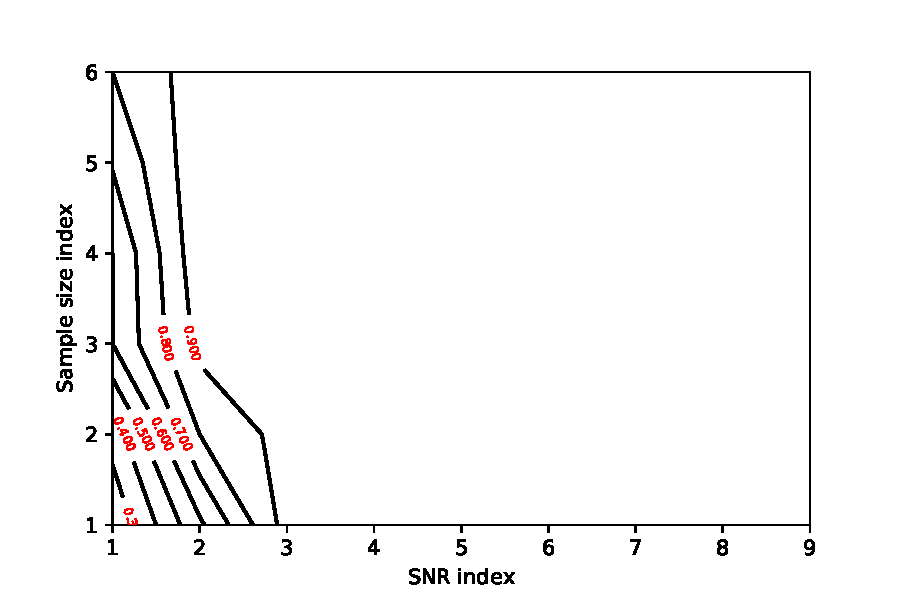
\includegraphics[width=\linewidth]{figure/aic_3.pdf}
			%\caption{fig1}
		\end{minipage}%
	}%
	\subfigure[AIC performance for $m=5$]{
		\begin{minipage}[t]{0.32\linewidth}
			\centering
			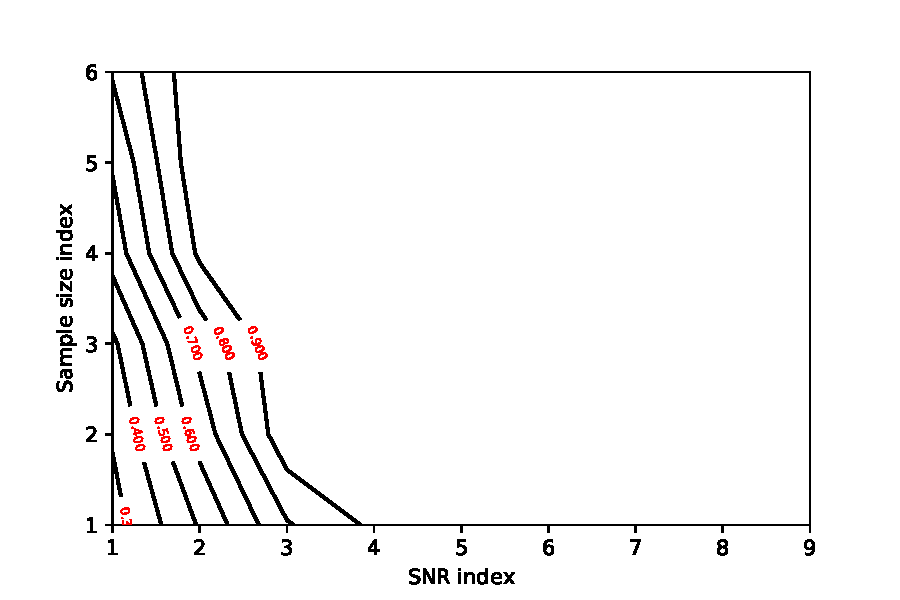
\includegraphics[width=\linewidth]{figure/aic_5.pdf}
			%\caption{fig2}
		\end{minipage}%
	}%
	\subfigure[AIC performance for $m=7$]{
		\begin{minipage}[t]{0.32\linewidth}
			\centering
			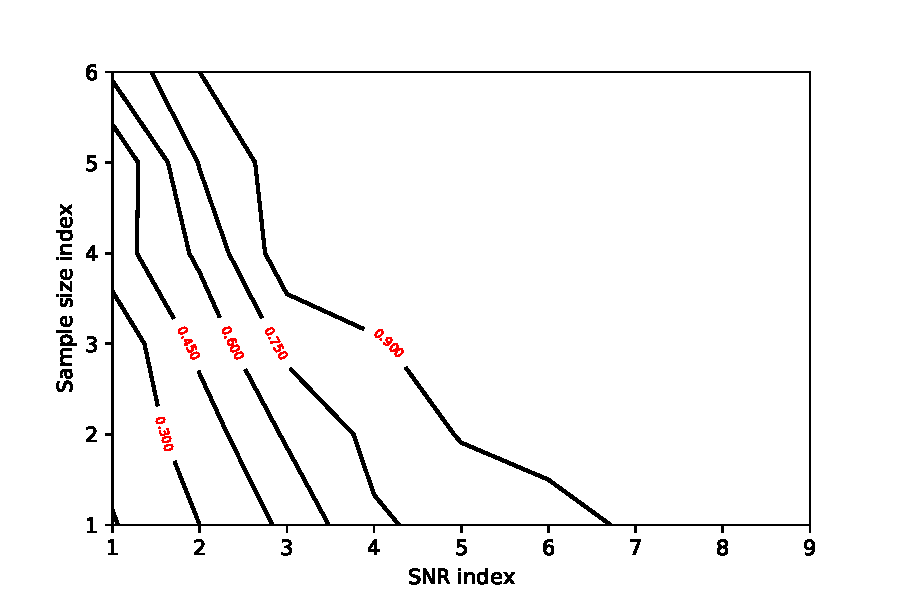
\includegraphics[width=\linewidth]{figure/aic_7.pdf}
			%\caption{fig2}
		\end{minipage}%
	}%
	
	\subfigure[BIC performance for $m=3$]{
		\begin{minipage}[t]{0.32\linewidth}
			\centering
			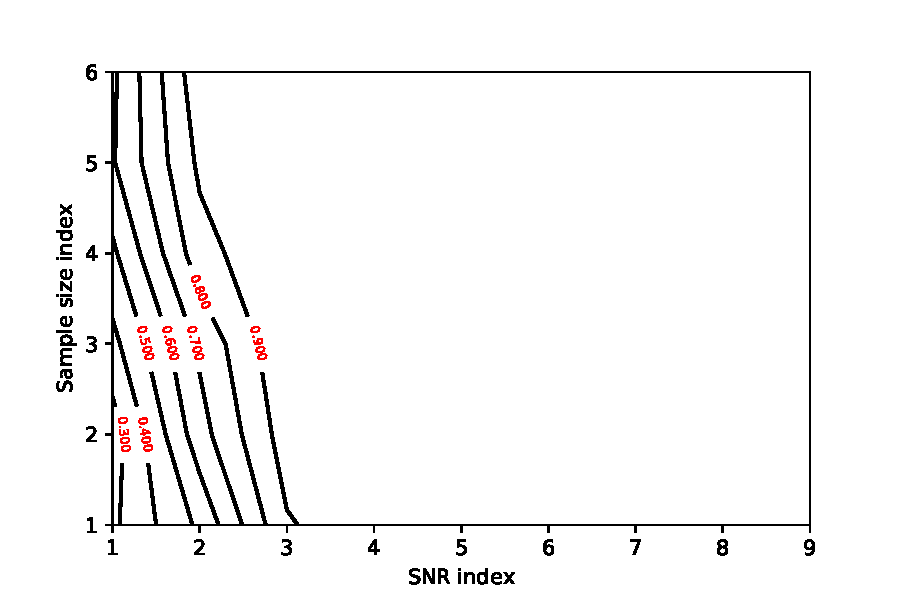
\includegraphics[width=\linewidth]{figure/bic_3.pdf}
			%\caption{fig1}
		\end{minipage}%
	}%
	\subfigure[BIC performance for $m=5$]{
		\begin{minipage}[t]{0.32\linewidth}
			\centering
			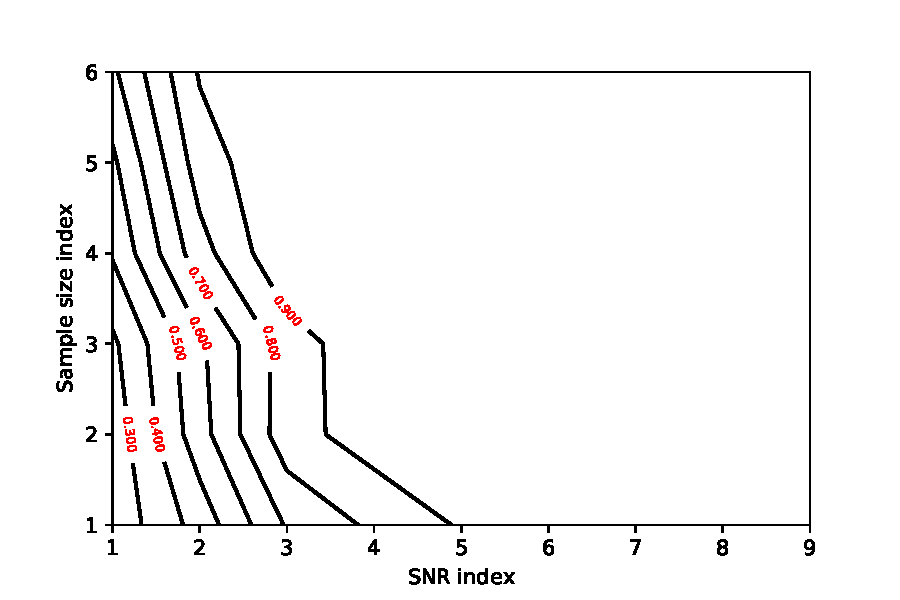
\includegraphics[width=\linewidth]{figure/bic_5.pdf}
			%\caption{fig2}
		\end{minipage}
	}%
	\subfigure[BIC performance for $m=7$]{
		\begin{minipage}[t]{0.32\linewidth}
			\centering
			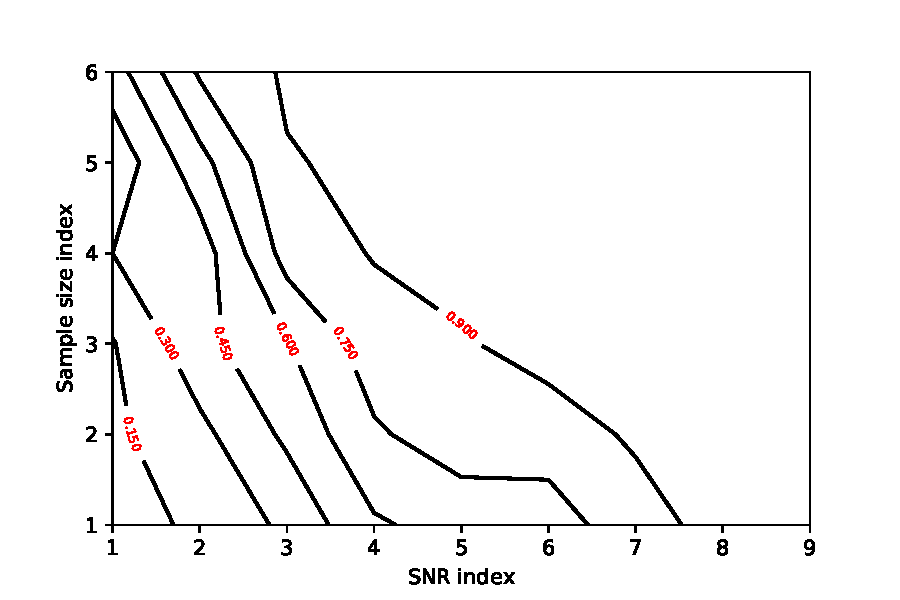
\includegraphics[width=\linewidth]{figure/bic_7.pdf}
			%\caption{fig2}
		\end{minipage}%
	}%
	
	\caption{Contour graphs of the experiment result}\label{fig:contour}
\end{figure}

It presents similar result to what presented in the lecture: when signal-noise ratio and sample size is small, AIC tends to perform a little better than BIC in terms of probability of successfully choosing the optimal model. What is different from the lecture is that when SNR and sample size is large (corresponding to the upper right area in the figure), AIC does not show any flaws (the diamond-like low-precision area vanishes). Another major observation is that when $m$ increases, the difficulty of selecting the optimal model also increases, namely the contours presenting a right shift and gentler slope. 
\section{Spectral clustering}
Use experiments to demonstrate that when spectral clustering works well, when it would fail. Summarize your results.

\textbf{Solution.} Here we present some comparisons between Spectral Clustering, K-means and Gaussian Mixture Model.
\begin{figure}[htbp]
	\centering
	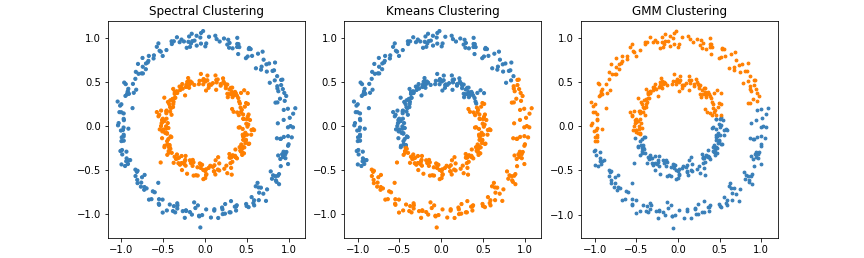
\includegraphics[width=0.8\textwidth]{figure/spectral_clustering_circle.png}
	\caption{Circled 2-D data}\label{fig:circle}
	
	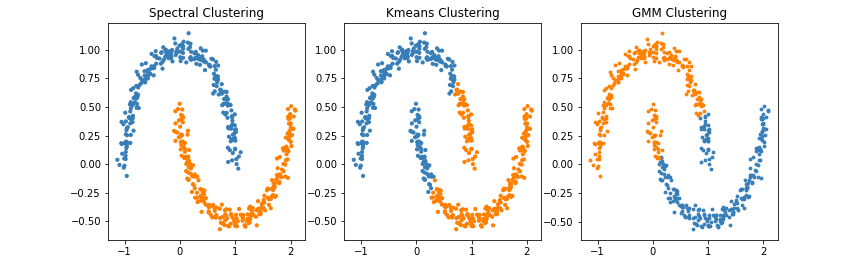
\includegraphics[width=0.8\textwidth]{figure/spectral_clustering_moon.png}
	\caption{Moon-like 2-D data}\label{fig:moon}
\end{figure}


Spectural clustering is designed for when we only know the pairwise similarity for datapoints, like in a social network or other graph-format data. It also suits for clusters that may not have a regular shape (as shown in Figure~\ref{fig:circle} and~\ref{fig:moon}), or manifolds in higher dimensions, as long as we carefully select the distance metric and covert the distaance matrix to similarity matrix, then to adjacency matrix. In this experimental setting, the conversion between similarity matrix and adjacency matrix is done by performing K nearest neighbors algorithm. This maight be tricky as we cna see in Figure~\ref{fig:gaussian} and~\ref{fig:sepagaussian}.
\begin{figure}[ht]
	\centering
	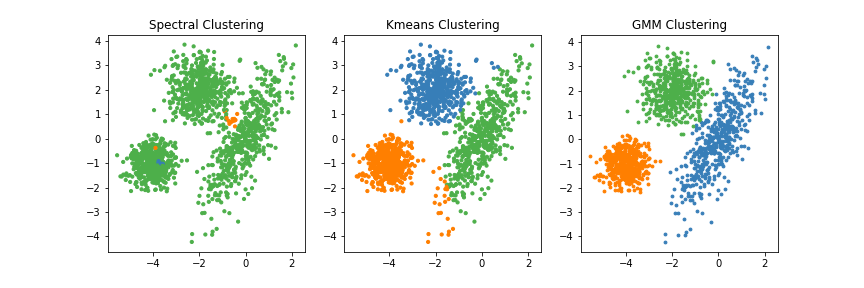
\includegraphics[width=0.8\textwidth]{figure/spectral_clustering_guassian.png}
	\caption{Gaussian Mixture 2-D data with clusters close to each other}\label{fig:gaussian}

	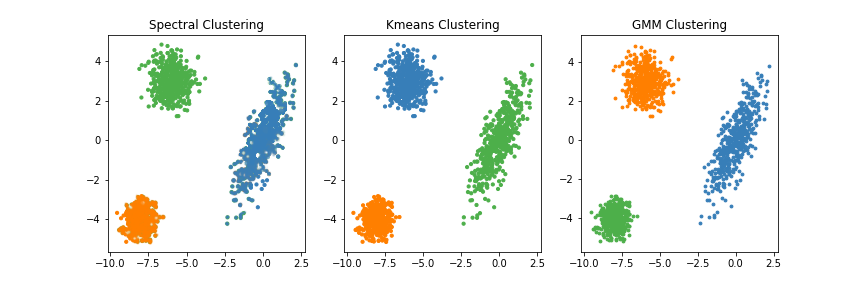
\includegraphics[width=0.8\textwidth]{figure/spectral_clustering_separatedguassian.png}
	\caption{Gaussian Mixture 2-D data with clusters separated from each other}\label{fig:sepagaussian}
\end{figure}

When the clusters are close enough (or even overlap in some scenario), we lack effective approach to construct adjacency matrixs such that spectral clustering can tell there are actually more than 1 clusters. Though spectral clustering fails in these scenario, do not forget what it is originally designed for and just don't expect everthing on a single method. 
\end{document}
